\chapter{Importations et exportations de données}

\section{Présentation}

Le logiciel Filo-Science intègre deux modules génériques permettant de réaliser soit des importations, soit des exportations. 
Le premier vise à importer des données de pistage de poissons ou des données transmises par des sondes d'analyse physico-chimique. Les données fournies sont de type tabulé (fichiers ressemblant à des fichiers CSV).
Le second sert à générer un export de données au format JSON, pouvant comprendre également les informations rattachées, pour pouvoir les réimporter dans une autre base de données.

Les tables qui permettent de décrire ces fonctions sont stockées dans le schéma \textit{import} (figure \ref{fig:export_schema}).
\begin{figure}[h!]
\begin{center}
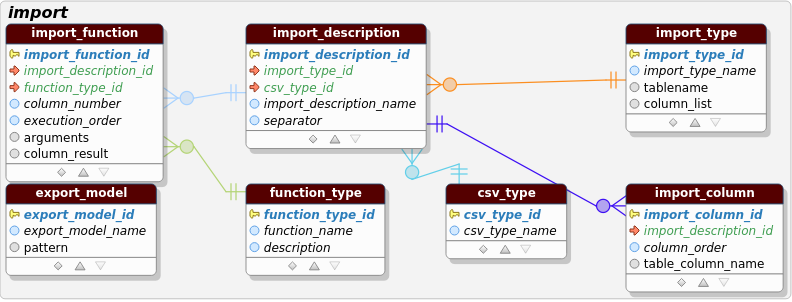
\includegraphics[width=\linewidth]{images/export_schema}
\captionof{figure}{Schéma des tables utilisées pour décrire les importations/exportations}
\label{fig:export_schema}
\end{center}
\end{figure}

\section{Importation de données tabulées}

Les structures des fichiers fournis par les systèmes d'acquisition automatique sont très variées, les données nécessitent souvent d'être reformatées ou recalculées avant de pouvoir être importées dans une table.

Le principe d'importation est le suivant :
\begin{itemize}
	\item chaque champ (une colonne) du fichier à importer peut faire l'objet d'une ou plusieurs transformations ou contrôles ;
	\item une fois l'ensemble de ces opérations réalisées, les champs pertinents vont être assignés à des colonnes de la table cible, et l'enregistrement réalisé en base de données.
\end{itemize}

\subsection{Types d'import}

Trois types d'import sont décrits et fournis, qui permettront d'alimenter les tables \textit{detection}, \textit{probe\_measure} et \textit{location}. 
La liste des colonnes utilisables pour l'importation est décrite, chaque colonne étant séparée par une virgule.

Les types d'import ne doivent pas être modifiés.

\subsection{Types de fonctions}

Les fonctions, codées dans l'application, sont décrites dans la table \textit{function\_type}. Cette table ne peut pas être modifiée.

La table \ref{tab:fonctions} présente la liste des fonctions utilisables pour préparer un import.

\begin{longtable}{|c|>{\raggedright\arraybackslash}p{5cm}|c|c|}
\caption{Liste des fonctions utilisées pour préparer un import.} \label{tab:fonctions} \\

\hline \multicolumn{1}{|c|}{\textbf{Nom de la fonction}} & \multicolumn{1}{c|}{\textbf{Description}} & \multicolumn{1}{c|}{\textbf{Contrôle ?}} & \multicolumn{1}{c|}{\textbf{Transformation ?}} \\ \hline 
\endfirsthead

\multicolumn{4}{c}%
{{\bfseries \tablename\ \thetable{} -- suite de la page précédente}} \\
\hline \multicolumn{1}{|c|}{\textbf{Nom de la fonction}} & \multicolumn{1}{c|}{\textbf{Description}} & \multicolumn{1}{c|}{\textbf{Contrôle ?}} & \multicolumn{1}{c|}{\textbf{Transformation ?}} \\ \hline 
\endhead

\hline \multicolumn{4}{|r|}{{Suite sur la page suivante}} \\ \hline
\endfoot

 \hline
\endlastfoot

testValue & Teste si un champ contient la valeur indiquée & X &  \\ 
getSecondsFromTime & Transforme un champ de type hh:mm:ss.u en ss.u &  & X \\ 
extractRightChar & Extrait les n caractères à droite du champ &  & X \\ 
concatenateDateAndTime & Concatène un champ date et un champ time. L'argument doit correspondre au numéro de la colonne time &  & X \\ 
transformJulianToDate & Transforme un nombre de jours depuis la date indiquée en référence (au format Y-m-d) en date exploitable au format Y-m-d &  & X \\ 
verifyTypeNumber & Vérifie si une valeur est numérique ou non & X &  \\ 
testColumnsNumber & Vérifie que le nombre de colonnes de la ligne courante correspond bien au nombre attendu &  & X \\ 
getIndividualFromTag & Récupère l'identifiant du poisson à partir du tag (RFID) &  & X \\ 
getIndividualFromTransmitter & Récupère l'identifiant du poisson à partir du transmetteur (radio ou acoustique) &  & X \\ 
numericToHexa & Transforme une valeur numérique en valeur Hexa, si celle-ci ne l'est pas. La valeur Hexa doit comprendre au moins une lettre.  &  & X \\ 
concatenate & Associe le contenu de colonnes ou du texte. L'argument doit être au format JSON, sous la forme : [{"type":"col","val":4}, {type:"str","val":":"}] &  &  \\ 
matchingCode & Remplace la valeur courante par une autre valeur, définie dans un argument JSON au format : {"valueSearched":correspondingValue, "2ndvalue":corresp2}. Pour la recherche des paramètres de sonde, valueSearched doit correspondre au libellé utilisé par la sonde, et correspondingValue à la valeur de la clé dans la table des paramètres &  & X \\ 
formatDateTime & Transforme une datetime dans un format reconnu par la base de données, à partir du format indiqué. Exemple : d/m/Y H:i:s pour une date de type 13/01/2019 08:50:00. La liste des formats autorisés est disponible ici : \href{https://www.php.net/manual/fr/datetime.createfromformat.php}{https://www.php.net/ manual/fr/datetime.createfromformat.php}&  & X \\ 
decodeAll & Transforme un jeu de caractère particulier en UTF-8. L'argument doit comprendre le jeu de caractère à transcoder, par exemple UTF-32. C'est l'ensemble de la ligne qui sera transcodé &  & X \\ 
transformDecimalSeparator & Transforme la virgule en point, pour les champs décimaux en français &  & X \\ 
\hline 

\end{longtable}

\subsection{Créer un modèle d'import}

Ouvrez le menu \textit{Télédétection > Paramètres > Modèles d'import}, puis cliquez sur le lien \textit{Nouveau modèle}. Les informations à renseigner sont les suivantes :
\begin{itemize}
	\item Type d'import : 
	\begin{itemize}
		\item Détection : données de détections enregistrées depuis une station fixe
		\item Données de sonde : relevés physico-chimiques réalisés par une sonde
		\item Détections manuelles : données de détection réalisées sur le terrain.
	\end{itemize}
	\item Type de fichier CSV :
	\begin{itemize}
		\item Data in columns : format classique des fichiers CSV. Une colonne contient toujours la même information
		\item Data in lines : chaque ligne décrit le paramètre relevé et la valeur associée
	\end{itemize}
	\item  Nom du modèle : nom mnémotechnique
	\item Séparateur de champs : indiquez le séparateur utilisé (point-virgule, virgule, tabulation, espace).
\end{itemize}

Une fois ces informations enregistrées, deux tableaux doivent être renseignés.

\subsubsection{Fonctions de test et de transformation}

Le premier contient la liste des fonctions de transformation ou de test à exécuter. Voici les paramètres à préciser pour chacune :
\begin{itemize}
	\item Nom de la fonction à exécuter : une fois sélectionnée, un texte décrivant son fonctionnement et les paramètres attendus est affiché
	\item N° de colonne à traiter : indiquez le numéro de la colonne sur laquelle va porter la fonction. Si la fonction porte sur plusieurs colonnes (concaténation, par exemple), indiquez le numéro de la première colonne
	\item N° de la colonne récupérant le résultat : s'il s'agit d'une fonction de transformation, indiquez dans quelle colonne le résultat va être stocké. Pour les fonctions de contrôle, indiquez la valeur 0 (aucun résultat n'est stocké)
	\item ordre d'exécution de la fonction : pour une même colonne, plusieurs fonctions peuvent être appelées successivement. Renseignez l'ordre d'exécution pour être sûr que le résultat correspondra à ce que vous attendez
	\item argument complémentaire : le cas échéant, indiquez la valeur attendue par la fonction pour s'exécuter. Le détail de la valeur est décrit dans l'explication de la fonction.
\end{itemize}

Si une fonction de contrôle échoue, la ligne ne sera pas traitée et sera indiquée comme telle lors de l'importation.

Il est possible d'exécuter plusieurs fonctions successives sur la même colonne.

À noter que certaines fonctions sont utilisées pour rechercher des identifiants présents dans la base de données à partir des informations fournies (numéros des poissons à partir des numéros des émetteurs, par exemple).

\subsubsection{Table d'équivalence entre les colonnes et les champs de la base de données}

Le second tableau à renseigner permet d'indiquer quelles colonnes doivent être insérées dans la base de données.
Voici les informations à indiquer :
\begin{itemize}
	\item le numéro de la colonne, telle qu'elle a été transformée après application de l'ensemble des fonctions décrites précédemment
	\item le nom du champ dans la base de données qui recevra l'information
	\item s'il s'agit d'un fichier où chaque élément est différent d'une ligne à l'autre (fichier de type Entité/relation), indiquez également si :
	\begin{itemize}
		\item le champ sert d'identifiant pour la valeur mesurée
		\item le champ contient la valeur mesurée
	\end{itemize}
\end{itemize}

\subsection{Exécuter un import}

Choisissez le menu \textit{Télédétection > Importation}, puis indiquez :
\begin{itemize}
	\item le fichier à importer
	\item le type d'import à réaliser
	\item le projet concerné
	\item s'il s'agit d'un import de données réalisées à partir d'une station fixe (antenne ou sonde), indiquez l'antenne ou la sonde concernée
	\item le mode \textit{test} permet d'exécuter toutes les opérations d'importation, sans réaliser la mise en base de données. Cela permet d'identifier les problèmes potentiels dans un fichier avant de réaliser l'opération de manière définitive
	\item en mode \textit{test}, le nombre de lignes à traiter doit être indiqué, ce qui permet de limiter la taille de l'échantillon à tester.
\end{itemize}

En mode test, deux tableaux sont produits : le premier présente les données prêtes à être importées, le second l'ensemble des messages d'erreur.

En mode normal, le premier tableau affiche le résultat de l'importation. Celui contenant les messages d'erreurs est identique.

\section{Export de données au format JSON}

Il est possible d'exporter un lot de données, réparties sur plusieurs tables, pour les réimporter dans une autre base de données. Par défaut, trois exports sont disponibles et intégrés directement dans l'application : export d'une campagne, d'une opération et de leurs données associées, et un export technique des modèles d'exports.

Les données sont exportées au format JSON.

\subsection{Description des modèles d'export}

Choisissez le menu \textit{Paramètres > Modèles d'export}. Hormis le nom du modèle, toutes les autres informations permettent de décrire les tables à exporter et les relations entre elles.

La saisie d'une nouvelle table passe par l'ajout d'un nouvel item dans la partie \textit{Description du modèle}. Chaque item peut être déplacé après création, si nécessaire.

Pour chaque table à exporter, voici les informations à renseigner :
\begin{itemize}
	\item nom de la table, telle qu'il figure dans la base de données
	\item alias de la table : si une même table peut être reliée à des tables parentes différentes, cette colonne devra être renseignée avec un nom différent pour chaque instance. C'est le cas notamment pour la table \textit{ambience}, qui peut être reliée soit à la table \textit{operation}, soit à la table \textit{sequence}.
	\item  clé primaire : indiquez la clé primaire utilisée dans la table. Elle ne doit pas être renseignée dans le cas d'une table porteuse d'une relation n-n, dont la clé est composée des clés des deux tables parentes (cas de la table \textit{operation\_operator}).
	\item clé métier : il s'agit de la colonne qui permet de retrouver de manière univoque un enregistrement dans la table. Selon les cas de figure, il peut s'agir :
	\begin{itemize}
		\item du libellé, pour une table de paramètres
		\item de la clé primaire elle-même, pour certaines tables de paramètres dont la clé est significative. Cela permet de conserver la valeur de cette clé, même si le libellé change
		\item du champ UUID, qui est un identifiant technique généré avec un algorithme garantissant qu'il est unique au niveau mondial. Cette valeur sera utilisée chaque fois qu'elle est disponible
	\end{itemize}
	\item clé étrangère : le nom du champ porteur de la relation avec le parent, qui contient donc la clé du parent
	\item la liste des champs de type booléen, en raison d'une particularité lors des importations liée à ceux-ci
	\item la liste des alias (ou du nom des tables) des tables filles
	\item dans le cas d'une table porteuse d'une relation n-n, c'est à dire dont la clé est composée des clés des deux tables parentes, il faudra indiquer :
	\begin{itemize}
		\item le nom du champ comprenant la seconde clé étrangère
		\item l'alias (ou le nom de la table) de la seconde table parente
	\end{itemize}
\end{itemize}

La première table présente dans la liste doit être la table principale de l'export. Les tables filles doivent être créées après leurs tables parentes.

Il est possible d'indiquer plusieurs tables principales (sans parents) dans le même modèle.

\subsection{Exporter des campagnes ou des opérations}

Depuis la liste des campagnes, ou depuis une campagne, cochez les lignes que vous voulez exporter, puis cliquez sur le bouton d'exportation. Le fichier JSON sera généré.

\subsection{Autres exportations}

Depuis la liste des modèles, il est possible de réaliser un export pour l'ensemble des données décrites dans un modèle.

Dans la liste, affichez le détail d'un des modèles, puis cliquez sur le bouton \textit{Exporter toutes les données concernées par le modèle}.

Attention : c'est une opération qui va traiter \underline{l'ensemble} d'une table et des données rattachées. Elle est à manipuler avec précaution, le volume des données générées peut être important.

\subsection{Importer un fichier JSON}

L'importation de campagnes ou d'opérations s'effectue au même endroit que leur exportation. Il suffit de sélectionner le fichier considéré pour qu'il soit importé.

Pour ces deux importations, le programme va travailler en mode \og remplace ou insert \fg{} : si un enregistrement est trouvé (à partir du champ métier), il est mis à jour, sinon il est créé.

Il est également possible de réaliser une importation rapide depuis le menu de création des modèles d'exportation, depuis le détail d'un modèle. Cette fonction peut être pratique pour mettre à jour des tables de référence.